\PassOptionsToPackage{unicode=true}{hyperref} % options for packages loaded elsewhere
\PassOptionsToPackage{hyphens}{url}
%
\documentclass[]{article}
\usepackage{lmodern}
\usepackage{amssymb,amsmath}
\usepackage{ifxetex,ifluatex}
\usepackage{fixltx2e} % provides \textsubscript
\ifnum 0\ifxetex 1\fi\ifluatex 1\fi=0 % if pdftex
  \usepackage[T1]{fontenc}
  \usepackage[utf8]{inputenc}
  \usepackage{textcomp} % provides euro and other symbols
\else % if luatex or xelatex
  \usepackage{unicode-math}
  \defaultfontfeatures{Ligatures=TeX,Scale=MatchLowercase}
\fi
% use upquote if available, for straight quotes in verbatim environments
\IfFileExists{upquote.sty}{\usepackage{upquote}}{}
% use microtype if available
\IfFileExists{microtype.sty}{%
\usepackage[]{microtype}
\UseMicrotypeSet[protrusion]{basicmath} % disable protrusion for tt fonts
}{}
\IfFileExists{parskip.sty}{%
\usepackage{parskip}
}{% else
\setlength{\parindent}{0pt}
\setlength{\parskip}{6pt plus 2pt minus 1pt}
}
\usepackage{hyperref}
\hypersetup{
            pdftitle={Informe 3},
            pdfauthor={Derek Corcoran, Giorgia Graells, Horacio Samaniego, Pablo Marquet},
            pdfborder={0 0 0},
            breaklinks=true}
\urlstyle{same}  % don't use monospace font for urls
\usepackage[margin=1in]{geometry}
\usepackage{longtable,booktabs}
% Fix footnotes in tables (requires footnote package)
\IfFileExists{footnote.sty}{\usepackage{footnote}\makesavenoteenv{longtable}}{}
\usepackage{graphicx,grffile}
\makeatletter
\def\maxwidth{\ifdim\Gin@nat@width>\linewidth\linewidth\else\Gin@nat@width\fi}
\def\maxheight{\ifdim\Gin@nat@height>\textheight\textheight\else\Gin@nat@height\fi}
\makeatother
% Scale images if necessary, so that they will not overflow the page
% margins by default, and it is still possible to overwrite the defaults
% using explicit options in \includegraphics[width, height, ...]{}
\setkeys{Gin}{width=\maxwidth,height=\maxheight,keepaspectratio}
\setlength{\emergencystretch}{3em}  % prevent overfull lines
\providecommand{\tightlist}{%
  \setlength{\itemsep}{0pt}\setlength{\parskip}{0pt}}
\setcounter{secnumdepth}{5}
% Redefines (sub)paragraphs to behave more like sections
\ifx\paragraph\undefined\else
\let\oldparagraph\paragraph
\renewcommand{\paragraph}[1]{\oldparagraph{#1}\mbox{}}
\fi
\ifx\subparagraph\undefined\else
\let\oldsubparagraph\subparagraph
\renewcommand{\subparagraph}[1]{\oldsubparagraph{#1}\mbox{}}
\fi

% set default figure placement to htbp
\makeatletter
\def\fps@figure{htbp}
\makeatother

\usepackage{booktabs}
\usepackage{longtable}
\usepackage{array}
\usepackage{multirow}
\usepackage{wrapfig}
\usepackage{float}
\usepackage{colortbl}
\usepackage{pdflscape}
\usepackage{tabu}
\usepackage{threeparttable}
\usepackage{threeparttablex}
\usepackage[normalem]{ulem}
\usepackage{makecell}
\usepackage{xcolor}

\title{Informe 3}
\author{Derek Corcoran, Giorgia Graells, Horacio Samaniego, Pablo Marquet}
\date{20/04/2020}

\begin{document}
\maketitle

\hypertarget{introducciuxf3n}{%
\section{Introducción}\label{introducciuxf3n}}

En este documento se mostrarán simulaciones destinadas a responder 3 puntos de la minuta solicitados por el ministerio de ciencia, basado en un modelo con conectividad espacial y estrucutrado por edades (Arenas et al. 2020), la modificación del modelo se encuentra explicada en detalle en Corcoran et al. (2020)

\begin{enumerate}
\def\labelenumi{\arabic{enumi}.}
\item
  Cuarentena total, las personas quedan con prohibición de salir de su casa, solo con permiso especiales.
\item
  Cuarentenas alternantes por comunas a nivel nacional de 15 días, las personas quedan con prohibición de salir de su casa 15 días (cuarentena) y luego 15 días con cierre de colegios y comercio. Una comuna entra en cuarentena cuando los casos llegan a 4 o 5 por 10.000.
\item
  Cierre de colegios y comercio.
\end{enumerate}

\hypertarget{simulaciones}{%
\section{Simulaciones}\label{simulaciones}}

Para todas las simulaciones se usaron el las funciones descritas y disponibles en Corcoran and Graells (2020), ahí también se encuentran las bases de datos con las que se realizaron estas simulaiciones

\hypertarget{extensiuxf3n-uxf3ptima-de-cuarentena-total.-simulaciuxf3n-del-15-abril-al-14-junio}{%
\subsection{Extensión óptima de cuarentena total. Simulación del 15 abril al 14 junio}\label{extensiuxf3n-uxf3ptima-de-cuarentena-total.-simulaciuxf3n-del-15-abril-al-14-junio}}

Para obtener la extensión óptima de una cuarentena total a nivel nacional se realizaron 12 simulaciones distintas que parten el día 20 de abril. Se consideraron 3 extensiones de cuarentena nacional (7, 15 y 30 días) y 3 valores de grado de confinamiento o \(\kappa_0\) distintos (0.5, 0.75 y 0.85, cada una representando cuarentenas con control leve, medio o fuerte). Para tener las condiciones iniciales del 20 de abril se modeló del 15 abril al 20 abril, manteniendo una cuarentena dinámica por comuna.

Estas simulaciones se contrastaron con una cuarentena dinámica la cual se gatilla cuando el número de infectados llega a 40/100,000 casos activos confirmados. Una vez gatillada la cuarentena, esta durará como mínimo 7 días, y al pasar los 7 días se observa la prevalencia nuevamente para determinar si la cuarentena se levanta o se renueva por otros 7 días

\hypertarget{inicio-uxf3ptimo-de-cuarentena-total}{%
\subsection{Inicio óptimo de cuarentena total}\label{inicio-uxf3ptimo-de-cuarentena-total}}

Determinación de fechas de inicio considerando extensión óptima definida

Esta parte asume que en la sección anterior se determinó la extensión optima que será simulada despúes de la cuarentena dinámica. Se simularán dos semanas sin cuarentena posterior a este periodo para ver los efectos.

\begin{itemize}
\item
  \begin{enumerate}
  \def\labelenumi{\arabic{enumi}.}
  \tightlist
  \item
    Desde el 15 abril cuarentena dinámica, 2. desde el 20 mayo cuarentena nacional por el número de días generado por la simulación anterior y 3. dos semanas sin cuarentena
  \end{enumerate}
\item
  \begin{enumerate}
  \def\labelenumi{\arabic{enumi}.}
  \tightlist
  \item
    Desde el 15 abril cuarentena dinámica, 2. desde el 1 mayo cuarentena nacional por el número de días generado por la simulación anterior y 3. dos semanas sin cuarentena
  \end{enumerate}
\item
  \begin{enumerate}
  \def\labelenumi{\arabic{enumi}.}
  \tightlist
  \item
    Desde el 15 abril cuarentena dinámica, 2. desde el 15 mayo cuarentena nacional por el número de días generado por la simulación anterior y 3. dos semanas sin cuarentena
  \end{enumerate}
\item
  \begin{enumerate}
  \def\labelenumi{\arabic{enumi}.}
  \tightlist
  \item
    Desde el 15 abril cuarentena dinámica, 2. desde el 30 mayo cuarentena nacional por el número de días generado por la simulación anterior y 3. dos semanas sin cuarentena
  \end{enumerate}
\end{itemize}

\hypertarget{resultados}{%
\section{Resultados}\label{resultados}}

\hypertarget{nivel-pauxeds}{%
\subsection{Nivel País}\label{nivel-pauxeds}}

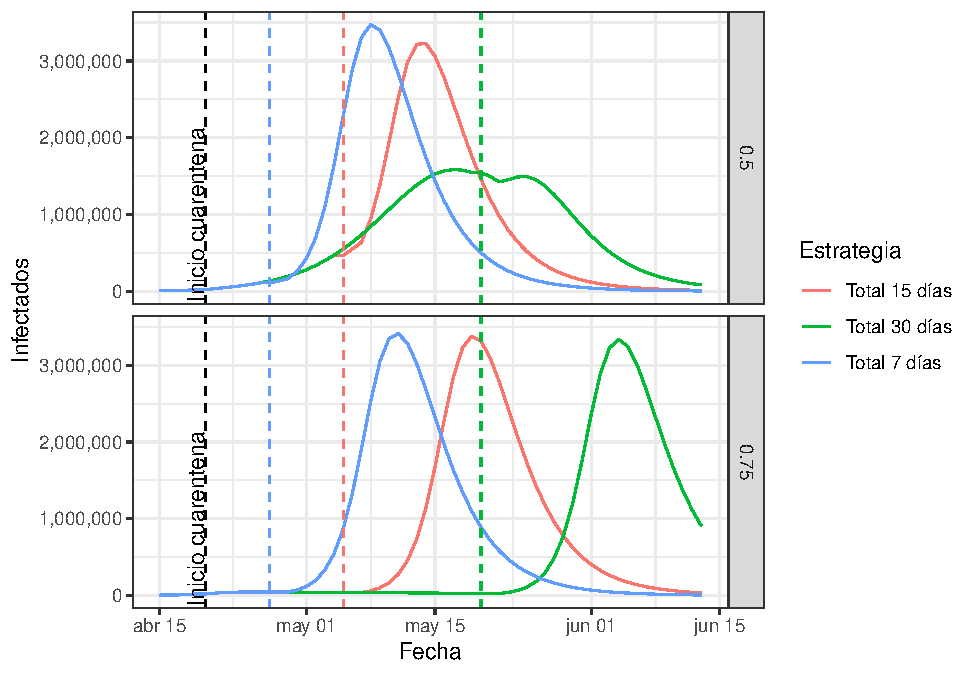
\includegraphics{Informe_Mesa_2020_04_16_files/figure-latex/unnamed-chunk-3-1.pdf}

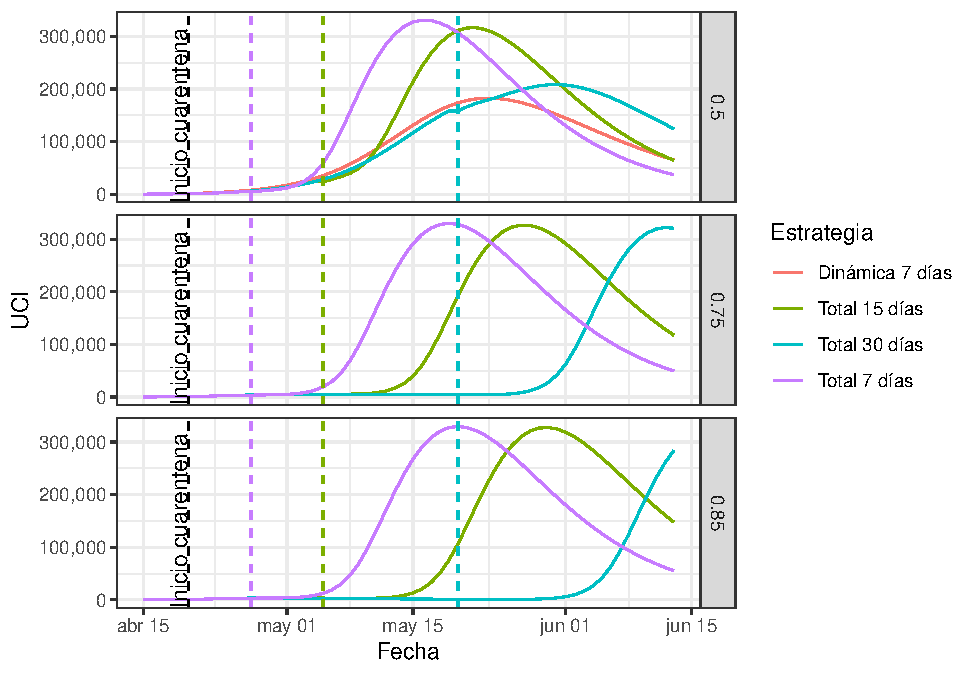
\includegraphics{Informe_Mesa_2020_04_16_files/figure-latex/unnamed-chunk-4-1.pdf}

\hypertarget{regiuxf3n-metropolitana}{%
\subsection{Región Metropolitana}\label{regiuxf3n-metropolitana}}

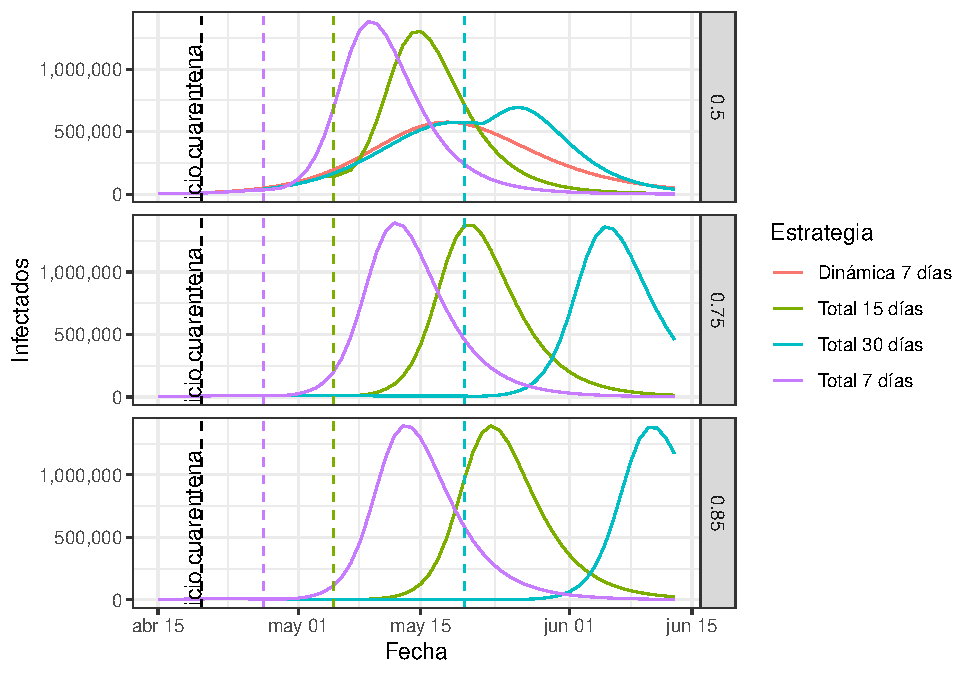
\includegraphics{Informe_Mesa_2020_04_16_files/figure-latex/unnamed-chunk-6-1.pdf}

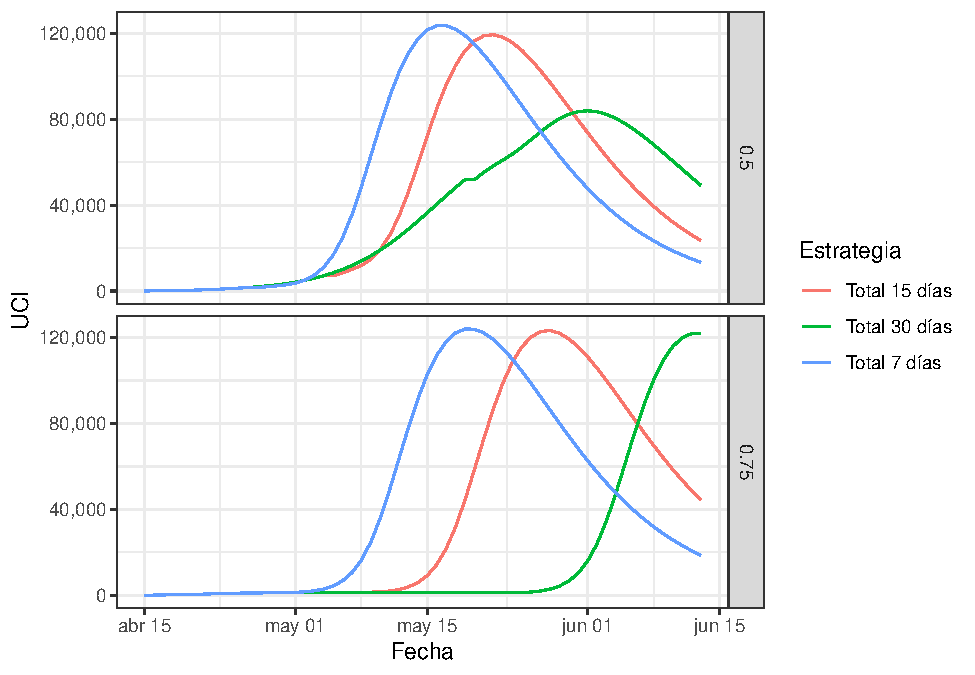
\includegraphics{Informe_Mesa_2020_04_16_files/figure-latex/unnamed-chunk-7-1.pdf}

\hypertarget{nivel-comunal-regiuxf3n-metropolitana}{%
\subsection{Nivel Comunal Región Metropolitana}\label{nivel-comunal-regiuxf3n-metropolitana}}

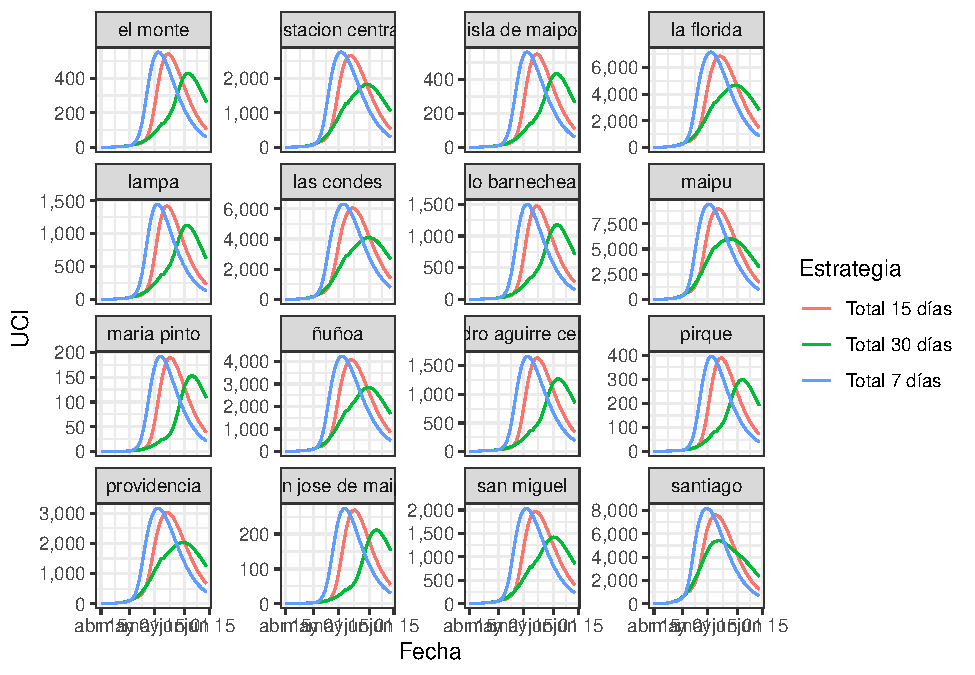
\includegraphics{Informe_Mesa_2020_04_16_files/figure-latex/unnamed-chunk-10-1.pdf}

\hypertarget{refs}{}
\leavevmode\hypertarget{ref-arenas2020mathematical}{}%
Arenas, Alex, Wesley Cota, Jesus Gomez-Gardenes, Sergio Gómez, Clara Granell, Joan T Matamalas, David Soriano-Panos, and Benjamin Steinegger. 2020. ``A Mathematical Model for the Spatiotemporal Epidemic Spreading of Covid19.'' \emph{medRxiv}. Cold Spring Harbor Laboratory Press.

\leavevmode\hypertarget{ref-derek_corcoran_barrios_2020_3756847}{}%
Corcoran, Derek, and Giorgia Graells. 2020. \emph{derek-corcoran-barrios/Covid19\_Chile\_Age: Modelo metapoblacional para simular el manejo de COVID19 en Chile} (version V1.0). Zenodo. \url{https://doi.org/10.5281/zenodo.3756847}.

\leavevmode\hypertarget{ref-corcoran_graells_2020}{}%
Corcoran, Derek, Giorgia Graells, Simón Castillo, Horacio Samaniego, and Pablo Marquet. 2020. ``Mplementación de Modelo Covid19 paraChile.'' \emph{Ecoinformatica}. \url{https://www.ecoinformatica.net/COVID19.html}.

\end{document}
